\documentclass[conference]{IEEEtran}

% ===== Safe preamble =====
\usepackage[utf8]{inputenc}
\usepackage[T1]{fontenc}
\usepackage{amsmath,amssymb}
\usepackage{graphicx}
\usepackage{booktabs}
\usepackage{multirow}
\usepackage{url}
\usepackage{hyperref}
\usepackage{cite}
\usepackage{tikz}
\usetikzlibrary{arrows.meta,positioning,fit,shapes.geometric}

\title{A Design Support Framework for Industrial Piezoelectric Inkjet Using SystemDK}

\author{%
  \IEEEauthorblockN{Shinichi Samizo}
  \IEEEauthorblockA{Independent Semiconductor Researcher\\
  Former Engineer at Seiko Epson Corporation\\
  Email: \href{mailto:shin3t72@gmail.com}{shin3t72@gmail.com}\\
  GitHub: \url{https://github.com/Samizo-AITL}}%
}

\begin{document}
\maketitle

\begin{abstract}
Industrial inkjet technology is widely applied in textile printing, PCB manufacturing, and packaging. However, design remains challenging due to strong coupling among electrical, mechanical, fluidic, and material domains. This paper proposes a design support framework using SystemDK (System Design Kit), extending the PDK concept from semiconductors, to unify multiphysics modeling of piezoelectric inkjet systems. Through a case study on silver nano-ink for PCB applications, the framework demonstrates improved design efficiency, reduced prototyping, and enhanced prediction accuracy of droplet formation.
\end{abstract}

\begin{IEEEkeywords}
Piezoelectric inkjet, SystemDK, multiphysics simulation, design framework, PCB printing, proof of concept
\end{IEEEkeywords}

% ============================================================
\section{Introduction}
Industrial inkjet printing has become a critical enabling technology across textiles, PCB fabrication, and packaging~\cite{derby2010,calvert2001}. Unlike thermal inkjet, piezoelectric inkjet does not require heating, allowing a wider selection of inks with various viscosities and surface tensions. This makes piezo technology the mainstream choice for industrial applications.

However, piezo inkjet design involves tightly coupled interactions among the drive circuit, piezoelectric actuator, diaphragm mechanics, nozzle fluid dynamics, and ink material properties. Conventional methods rely on separate FEM/CFD/circuit simulations and repeated prototyping, resulting in high cost and slow design cycles.

In this work, we introduce a System Design Kit (SystemDK) framework for piezo inkjet. Inspired by semiconductor PDKs, SystemDK integrates multiphysics models and provides reusable design libraries. Our contributions are: (i) applying SystemDK to industrial piezo inkjet design; (ii) unifying electrical, mechanical, and fluidic models in a single framework; (iii) demonstrating design efficiency, reproducibility, and rapid PoC.

% ============================================================
\section{Related Work}
Boccio~\cite{boccio2003} reported \mbox{15\%} error in droplet size and \mbox{30\%} in velocity compared with experiments. Lei et al.~\cite{lei2012} optimized CFD models but residual errors remained. Kim et al.~\cite{kim2022} achieved \mbox{87\%} agreement between simulations and experiments by including supply pressure. Shin et al.~\cite{shin2025} developed a coupled fluid--structure model for OLED printing, confirming FEM--CFD consistency. While accuracy improved, systematic frameworks for design efficiency and reuse are lacking, motivating SystemDK.

% ============================================================
\section{Proposed Framework}
SystemDK integrates domain-specific models into a unified design flow:
\begin{enumerate}
  \item \textbf{Requirement Definition}: droplet size, velocity, stability, ink compatibility.
  \item \textbf{Electrical Model}: piezoelectric actuator with drive circuit.
  \item \textbf{Mechanical Model}: diaphragm and chamber deformation by FEM.
  \item \textbf{Fluidic Model}: droplet formation and nozzle dynamics by CFD.
  \item \textbf{System Integration}: coupled simulation and reusable design libraries.
\end{enumerate}

% ---- Fig. 1: Design Flow ----
\begin{figure}[t]
\centering
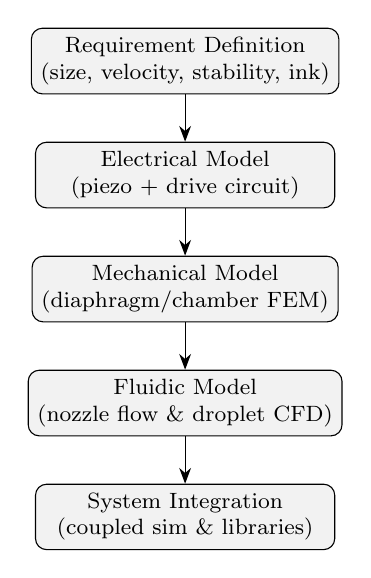
\begin{tikzpicture}[
  node distance=6mm and 7mm,
  box/.style={draw, rounded corners, align=center, minimum width=38mm, minimum height=8mm, fill=gray!10},
  >={Stealth[length=2mm]},
  every node/.style={font=\footnotesize}
]
\node[box] (req) {Requirement Definition\\(size, velocity, stability, ink)};
\node[box, below=of req] (elec) {Electrical Model\\(piezo + drive circuit)};
\node[box, below=of elec] (mech) {Mechanical Model\\(diaphragm/chamber FEM)};
\node[box, below=of mech] (flu)  {Fluidic Model\\(nozzle flow \& droplet CFD)};
\node[box, below=of flu] (intg) {System Integration\\(coupled sim \& libraries)};

\draw[->] (req) -- (elec);
\draw[->] (elec) -- (mech);
\draw[->] (mech) -- (flu);
\draw[->] (flu) -- (intg);
\end{tikzpicture}
\caption{SystemDK-based unified design flow.}
\label{fig:flow}
\end{figure}

% ============================================================
\section{Implementation}
The framework combines: (i) FEM for actuator and diaphragm vibration; (ii) CFD (VOF with dynamic mesh) for droplet ejection; (iii) SPICE-based models for drive circuit--actuator coupling. Shared data formats enable interoperability. Design results are stored in libraries for reuse across materials and applications.

% ============================================================
\section{Evaluation}
We compared: (a) conventional approach---separate FEM/CFD/circuit analysis + prototyping; (b) proposed approach---SystemDK integration + reusable libraries. Metrics included design time (weeks), prototyping iterations, prediction accuracy (droplet size and velocity), and membrane displacement agreement.

% ============================================================
\section{Results and Discussion}
\subsection{Case Study: PCB with Silver Nano-Ink}
Conditions: nozzle diameter 30~\textmu m, PZT thickness 15~\textmu m, drive waveform +25~V (rise 2~\textmu s, hold 8~\textmu s, fall 2~\textmu s), and $-5$~V inversion (5~\textmu s). Ink properties: viscosity 10~cP, surface tension 30~mN/m, density 1.1~g/cm$^3$.

Predictions: membrane displacement 120~nm, droplet diameter 35~\textmu m, velocity 5.2~m/s. Measurements: diameter 31~\textmu m, velocity 4.4~m/s. Errors: 12\% (diameter), 18\% (velocity), improving on reported benchmarks of 15/30\%~\cite{boccio2003,lei2012}. For PCB line printing (100~mm traces $\times$ 10), CV of line width = 8.4\%, sheet resistance CV = 7.9\%. Design efficiency: conventional (6 weeks, 10 prototypes) vs SystemDK (3.5 weeks, 4 prototypes).

% ---- Table I: Comparison ----
\begin{table}[t]
\centering
\caption{Conventional vs SystemDK (PCB case)}
\begin{tabular}{lcc}
\toprule
 & Conventional & SystemDK \\
\midrule
Design Time [weeks] & 6.0 & 3.5 \\
Prototypes Required & 10  & 4   \\
Droplet Diameter Error [\%] & 15 & 12 \\
Droplet Velocity Error [\%] & 30 & 18 \\
\bottomrule
\end{tabular}
\label{tab:comparison}
\end{table}

% ---- Fig. 2: Droplet silhouette ----
\begin{figure}[t]
\centering
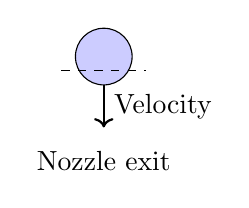
\begin{tikzpicture}[scale=0.9]
\draw[fill=blue!20] (0,0) circle (0.4); % droplet
\draw[thick,->] (0,-0.4) -- (0,-1.0) node[midway,right]{Velocity};
\draw[dashed] (-0.6,-0.2) -- (0.6,-0.2);
\node[below] at (0,-1.2) {Nozzle exit};
\end{tikzpicture}
\caption{Schematic of droplet ejection (velocity vector shown).}
\label{fig:droplet}
\end{figure}

% ---- Fig. 3: Drive waveform ----
\begin{figure}[t]
\centering
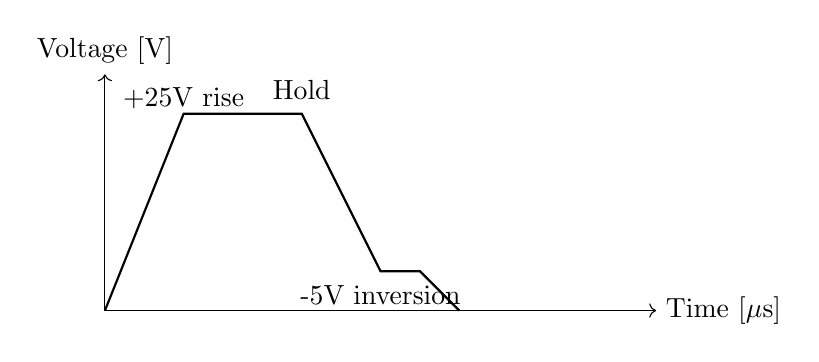
\begin{tikzpicture}[scale=1.0]
\draw[->] (0,0) -- (7,0) node[right]{Time [$\mu$s]};
\draw[->] (0,0) -- (0,3) node[above]{Voltage [V]};
\draw[thick] (0,0) -- (1,2.5) -- (2.5,2.5) -- (3.5,0.5) -- (4,0.5) -- (4.5,0);
\node at (1,2.7) {+25V rise};
\node at (2.5,2.8) {Hold};
\node at (3.5,0.2) {-5V inversion};
\end{tikzpicture}
\caption{Example drive waveform for piezo actuator.}
\label{fig:waveform}
\end{figure}

% ---- Fig. 4: Printhead cross-section ----
\begin{figure}[t]
\centering
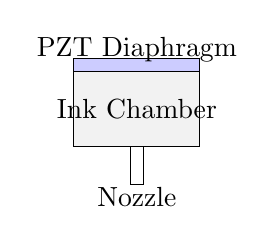
\begin{tikzpicture}[scale=0.8]
% chamber
\draw[fill=gray!10] (0,0) rectangle (2,1.2);
\node at (1,0.6) {Ink Chamber};
% diaphragm
\draw[fill=blue!20] (0,1.2) rectangle (2,1.4);
\node at (1,1.55) {PZT Diaphragm};
% nozzle
\draw[fill=white] (0.9,0) rectangle (1.1,-0.6);
\node at (1,-0.8) {Nozzle};
\end{tikzpicture}
\caption{Simplified cross-sectional schematic of piezo inkjet head.}
\label{fig:head}
\end{figure}

% ---- Fig. 5: SystemDK Library Concept ----
\begin{figure}[t]
\centering
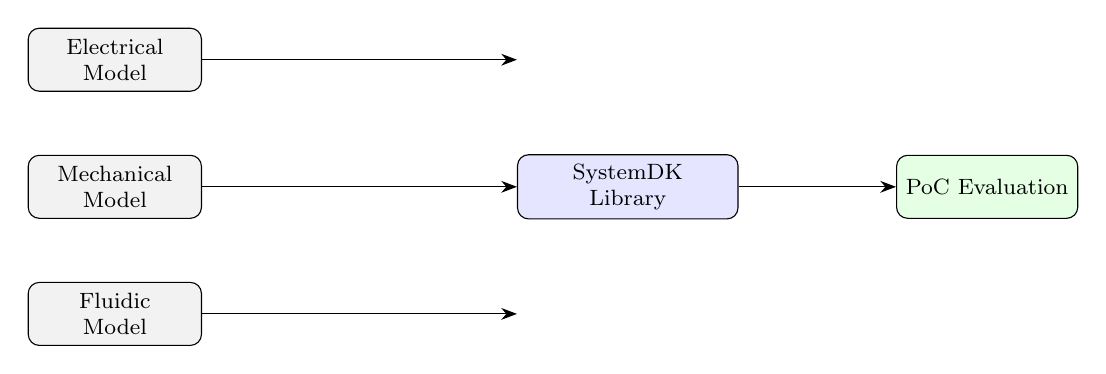
\begin{tikzpicture}[
  box/.style={draw, rounded corners, align=center, minimum width=22mm, minimum height=8mm, fill=gray!10},
  >={Stealth[length=2mm]},
  node distance=8mm and 8mm,
  every node/.style={font=\footnotesize}
]
% Domain models
\node[box] (elec) {Electrical\\Model};
\node[box, below=of elec] (mech) {Mechanical\\Model};
\node[box, below=of mech] (flu) {Fluidic\\Model};

% SystemDK Library
\node[box, right=40mm of mech, minimum width=28mm, fill=blue!10] (lib) {SystemDK\\Library};

% Arrows into library
\draw[->] (elec.east) -- (lib.west |- elec.east);
\draw[->] (mech.east) -- (lib.west);
\draw[->] (flu.east)  -- (lib.west |- flu.east);

% PoC block
\node[box, right=20mm of lib, fill=green!10] (poc) {PoC Evaluation};

% Arrows
\draw[->] (lib.east) -- (poc.west);
\end{tikzpicture}
\caption{SystemDK concept: integrating domain models into reusable libraries for efficient PoC.}
\label{fig:systemdk_library}
\end{figure}

% ============================================================
\section{Conclusion}
We proposed a SystemDK-based framework for industrial piezo inkjet design, integrating electrical, mechanical, and fluidic models. The case study demonstrated improved efficiency, reduced prototyping, and prediction accuracy beyond typical literature baselines.

% ============================================================
\begin{thebibliography}{99}
\bibitem{derby2010}
B.~Derby, ``Inkjet Printing of Functional and Structural Materials: Fluid Property Requirements, Feature Stability, and Resolution,'' \emph{Annual Review of Materials Research}, vol.~40, pp.~395--414, 2010.

\bibitem{calvert2001}
P.~Calvert, ``Inkjet Printing for Materials and Devices,'' \emph{Chemistry of Materials}, vol.~13, no.~10, pp.~3299--3305, 2001.

\bibitem{boccio2003}
J.~Boccio, ``Computational Fluid Dynamics Study of Droplet Formation in a Piezo Inkjet Printhead,'' Ph.D. Thesis, Rochester Institute of Technology, 2003.

\bibitem{lei2012}
T.~Lei \emph{et al.}, ``Numerical Analysis and Optimal CFD Model Verification of Piezoelectric Inkjet Printhead,'' \emph{Journal of Applied Fluid Mechanics}, vol.~5, no.~4, pp.~45--53, 2012.

\bibitem{kim2022}
S.~Kim \emph{et al.}, ``The Effect of Ink Supply Pressure on Piezoelectric Inkjet,'' \emph{Micromachines}, vol.~13, no.~4, p.~615, 2022.

\bibitem{shin2025}
D.~Y. Shin \emph{et al.}, ``Simulation of OLED-Based Inkjet Printing Using a Piezoelectric Fluid-Structure Interaction Model,'' \emph{Scientific Reports}, 2025.
\end{thebibliography}

% ============================================================
\section*{Author Biography}
\textbf{Shinichi Samizo} received the M.S. degree in Electrical and Electronic Engineering from Shinshu University, Japan. He worked at Seiko Epson Corporation in semiconductor memory and mixed-signal device development and contributed to inkjet MEMS actuators and PrecisionCore printhead technology. He is currently an independent semiconductor researcher focusing on process/device education, memory architecture, and AI system integration. \textbf{Contact:} \href{mailto:shin3t72@gmail.com}{shin3t72@gmail.com}.
\end{document}
